\documentclass[tikz,border=8pt]{standalone}
\usepackage{tikz}
\usepackage{fontawesome5}
\usepackage{amsmath,amssymb}
\usetikzlibrary{arrows.meta,positioning,fit,backgrounds,calc,shadows,shapes.geometric}

% Lavender Color Palette
\definecolor{lavenderDark}{RGB}{15, 44, 89}
\definecolor{lavenderDeep}{RGB}{10, 28, 58}
\definecolor{lavenderMedium}{RGB}{29, 78, 158}
\definecolor{lavenderLight}{RGB}{240, 246, 255}
\definecolor{lavenderBorder}{RGB}{180, 205, 237}
\definecolor{lavenderAccent}{RGB}{2, 132, 199}
\definecolor{prismNavy}{RGB}{15, 44, 89}
\definecolor{prismBlue}{RGB}{29, 78, 158}
\definecolor{prismTeal}{RGB}{13, 148, 136}
\definecolor{prismMint}{RGB}{236, 253, 245}
\definecolor{prismGold}{RGB}{217, 119, 6}
\definecolor{prismDark}{RGB}{15, 23, 42}
\definecolor{prismLight}{RGB}{248, 250, 252}

\begin{document}
% End-to-End System Flow for Deep Learning Ear Disease Detection
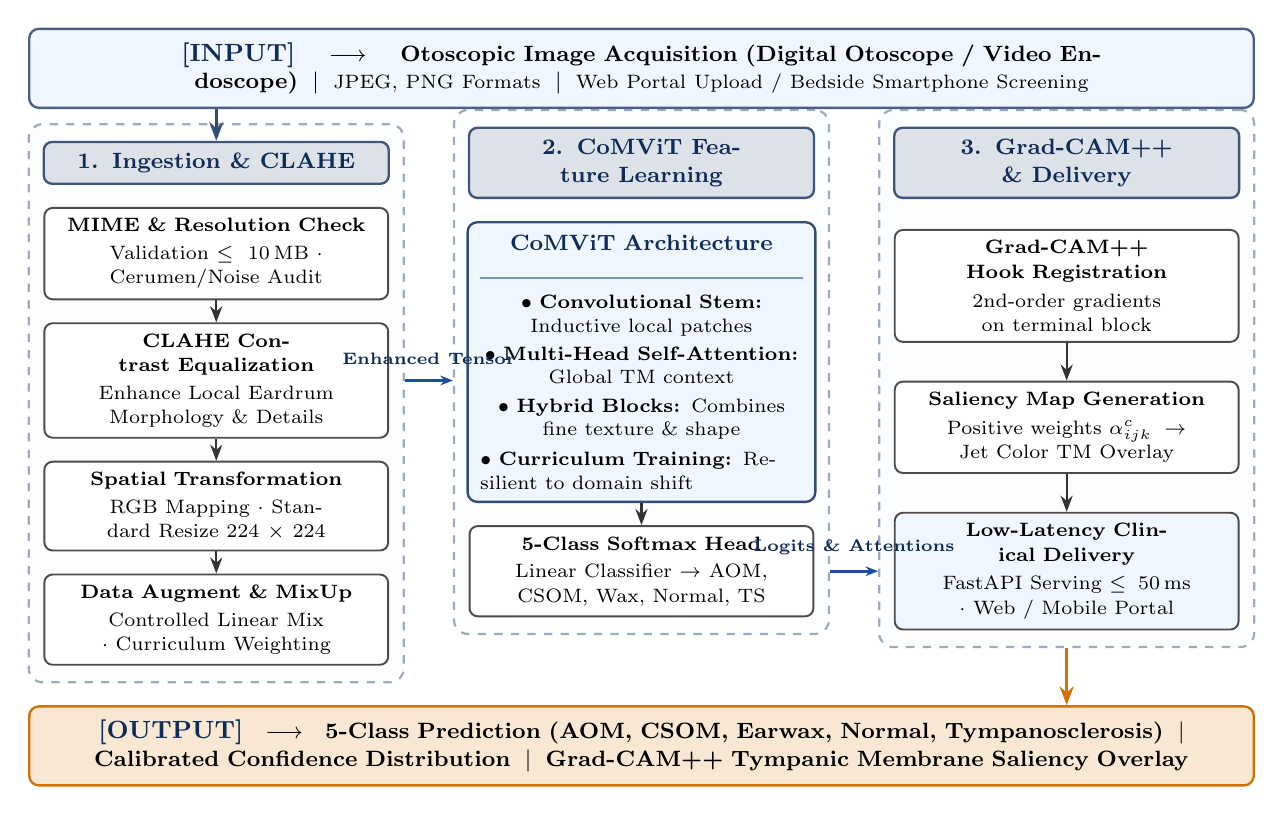
\begin{tikzpicture}[
    x=1cm, y=1cm,
    font=\sffamily,
    inout/.style={
        rectangle, rounded corners=3.5pt, line width=0.85pt,
        inner sep=5pt, align=center,
        font=\fontsize{8.2}{9.8}\selectfont
    },
    hdrbox/.style={
        rectangle, draw=lavenderDark!80, line width=0.85pt, fill=lavenderDark!14,
        rounded corners=3pt, inner sep=4pt, align=center,
        text width=4.10cm,
        font=\fontsize{8.5}{10.2}\selectfont\bfseries\color{lavenderDark}
    },
    stepbox/.style={
        rectangle, draw=black!70, line width=0.7pt, fill=white,
        rounded corners=3pt, inner sep=3.8pt, align=center,
        text width=4.10cm,
        font=\fontsize{7.5}{8.8}\selectfont
    },
    enginebox/.style={
        rectangle, draw=lavenderDark!85, line width=0.85pt, fill=lavenderLight,
        rounded corners=3.5pt, inner sep=4.5pt, align=left,
        text width=4.10cm,
        font=\fontsize{7.2}{8.8}\selectfont
    },
    stagebox/.style={
        rectangle, draw=lavenderDark!40, dashed, rounded corners=5pt, line width=0.8pt,
        fill=lavenderLight!25, inner xsep=5pt, inner ysep=6pt
    },
    flowarr/.style={
        -{Stealth[scale=0.85]}, line width=0.85pt, draw=black!80
    },
    transarr/.style={
        -{Stealth[length=4.5pt, width=3.5pt]}, line width=1.1pt, draw=lavenderMedium
    }
]

    % 1. TOP: INPUT BAR
    \node [inout, fill=lavenderLight, draw=lavenderDark!75, text width=15.2cm] (input_node) at (0, 3.40) {
        \textbf{\fontsize{8.8}{10.4}\selectfont\color{lavenderDark}[INPUT]} $\;\longrightarrow\;$
        \textbf{Otoscopic Image Acquisition (Digital Otoscope / Video Endoscope)}\; $\vert$\;
        {\fontsize{7.2}{8.5}\selectfont JPEG, PNG Formats}\; $\vert$\;
        {\fontsize{7.2}{8.5}\selectfont Web Portal Upload / Bedside Smartphone Screening}
    };

    % 2. MIDDLE: 3-STAGE HORIZONTAL PIPELINE

    % --- STAGE 1: INGESTION & PREPROCESSING ---
    \node [hdrbox] (h1) at (-5.40, 2.20) {1. Ingestion \& CLAHE};
    \node [stepbox, below=0.28cm of h1] (s1_1) {
        \textbf{MIME \& Resolution Check}\\[0.15em]
        {\fontsize{6.8}{8.0}\selectfont Validation $\le 10$\,MB $\cdot$ Cerumen/Noise Audit}
    };
    \node [stepbox, below=0.28cm of s1_1] (s1_2) {
        \textbf{CLAHE Contrast Equalization}\\[0.15em]
        {\fontsize{6.8}{8.0}\selectfont Enhance Local Eardrum Morphology \& Details}
    };
    \node [stepbox, below=0.28cm of s1_2] (s1_3) {
        \textbf{Spatial Transformation}\\[0.15em]
        {\fontsize{6.8}{8.0}\selectfont RGB Mapping $\cdot$ Standard Resize $224\times 224$}
    };
    \node [stepbox, below=0.28cm of s1_3] (s1_4) {
        \textbf{Data Augment \& MixUp}\\[0.15em]
        {\fontsize{6.8}{8.0}\selectfont Controlled Linear Mix $\cdot$ Curriculum Weighting}
    };

    \draw [flowarr] (s1_1) -- (s1_2);
    \draw [flowarr] (s1_2) -- (s1_3);
    \draw [flowarr] (s1_3) -- (s1_4);

    \begin{scope}[on background layer]
    \node [stagebox, fit=(h1) (s1_4)] (stage1) {};
    \end{scope}

    % --- STAGE 2: COMVIT INFERENCE ---
    \node [hdrbox] (h2) at (0, 2.20) {2. CoMViT Feature Learning};
    \node [enginebox, below=0.28cm of h2] (s2_1) {
        \centering\textbf{\fontsize{8.0}{9.5}\selectfont\color{lavenderDark}CoMViT Architecture}\\[0.2em]
        {\color{lavenderMedium!60}\rule{\linewidth}{0.5pt}}\\[0.28em]
        {\fontsize{7.0}{8.5}\selectfont
        $\bullet$ \textbf{Convolutional Stem:} Inductive local patches\\[0.22em]
        $\bullet$ \textbf{Multi-Head Self-Attention:} Global TM context\\[0.22em]
        $\bullet$ \textbf{Hybrid Blocks:} Combines fine texture \& shape\\[0.22em]
        $\bullet$ \textbf{Curriculum Training:} Resilient to domain shift}
    };

    \node [stepbox, below=0.28cm of s2_1] (s2_2) {
        \textbf{5-Class Softmax Head}\\[0.15em]
        {\fontsize{6.8}{8.0}\selectfont Linear Classifier $\to$ AOM, CSOM, Wax, Normal, TS}
    };

    \draw [flowarr] (s2_1) -- (s2_2);

    \begin{scope}[on background layer]
    \node [stagebox, fit=(h2) (s2_2)] (stage2) {};
    \end{scope}

    % --- STAGE 3: GRAD-CAM++ & DELIVERY ---
    \node [hdrbox] (h3) at (5.40, 2.20) {3. Grad-CAM++ \& Delivery};
    \node [stepbox, below=0.38cm of h3] (s3_1) {
        \textbf{Grad-CAM++ Hook Registration}\\[0.2em]
        {\fontsize{6.8}{8.0}\selectfont 2nd-order gradients on terminal block}
    };
    \node [stepbox, below=0.48cm of s3_1] (s3_2) {
        \textbf{Saliency Map Generation}\\[0.2em]
        {\fontsize{6.8}{8.0}\selectfont Positive weights $\alpha_{ijk}^c \to$ Jet Color TM Overlay}
    };
    \node [stepbox, below=0.48cm of s3_2, fill=lavenderLight] (s3_3) {
        \textbf{Low-Latency Clinical Delivery}\\[0.2em]
        {\fontsize{6.8}{8.0}\selectfont FastAPI Serving $\le 50$\,ms $\cdot$ Web / Mobile Portal}
    };

    \draw [flowarr] (s3_1) -- (s3_2);
    \draw [flowarr] (s3_2) -- (s3_3);

    \begin{scope}[on background layer]
    \node [stagebox, fit=(h3) (s3_3)] (stage3) {};
    \end{scope}

    % Transition arrows between stages
    \draw [transarr] (stage1.east |- s1_2) -- 
        node[above=2pt, font=\fontsize{6.0}{7.0}\selectfont\bfseries\color{lavenderDark}]{Enhanced Tensor} (stage2.west |- s1_2);

    \draw [transarr] (stage2.east |- s2_2) -- 
        node[above=2pt, font=\fontsize{6.0}{7.0}\selectfont\bfseries\color{lavenderDark}]{Logits \& Attentions} (stage3.west |- s2_2);

    \draw [flowarr, line width=1.1pt, draw=lavenderDark!85] (input_node.south -| h1.north) -- (h1.north);

    % 3. BOTTOM: OUTPUT BAR
    \node [inout, fill=prismGold!18, draw=prismGold!95!black, text width=15.2cm, below=0.50cm of $(stage1.south)!0.5!(stage3.south)$] (output_node) {
        \textbf{\fontsize{8.8}{10.4}\selectfont\color{lavenderDark}[OUTPUT]} $\;\longrightarrow\;$
        \textbf{5-Class Prediction (AOM, CSOM, Earwax, Normal, Tympanosclerosis)}\; $\vert$\;
        \textbf{Calibrated Confidence Distribution}\; $\vert$\;
        \textbf{Grad-CAM++ Tympanic Membrane Saliency Overlay}
    };

    \draw [flowarr, line width=1.1pt, draw=prismGold!95!black] (stage3.south -| h3.south) -- (output_node.north -| h3.south);

\end{tikzpicture}
\end{document}
